\section{Processes}

When you run a program, the OS creates a process to execute the program in. A process is an illusion created by the OS. It is an execution environment for a program. This environment gives the program limited rights (access, name spaces, threads, etc.) and therefore it is both a security and a resource principal.


\subsection{Creating a Process}

There are two main approaches to creating new processes:

\begin{itemize}
	\item \textbf{Spawn} - constructs a running process from scratch
	\item \textbf{Fork / Exec} - creates a copy of the calling process or replaces the current program with another in the same process
\end{itemize}

\textbf{Spawn}

\begin{itemize}
	\item Create and initialize the process control block (PCB) in the kernel
	\item Create and initialize a new address space
	\item Load the program into the address space
	\item Copy arguments into memory in the address space
	\item Initialize the hardware context to start execution at "start"
	\item Inform the scheduler that the new process is ready to run
\end{itemize}

Spawn is very complex, we have to specify everything about the new environment. If we omit a key argument a new process might have insufficient rights or resources or it might fail to function due to a security fault. \medskip

\textbf{Fork}

Fork on the other hand is less complex. The child process is almost an exact copy of the parent, with a different PID. We know which process we are in from the return value of the \textit{fork()} call ($0$ for child, $>0$ for parent, $<0$ for error). The complete UNIX process management API also includes:

\begin{itemize}
	\item \textit{exec()} - system call to change the program being run by the current process
	\item \textit{wait()} - system call to wait for a process to finish
	\item \textit{signal()} - system call to send a notification to another process
\end{itemize}

In contrast to \textit{spawn()}, here the child revokes rights and access explicitly before \textit{exec()}, further we can use the full kernel API to customize the execution environment.


\subsection{The Process Control Block}

The PCB is the main kernel data structure used to represent a process. It has to hold or refer to the page table, trap frame, kernel stack, open files, program name, scheduling state, PID, etc.


\subsection{Process Context Switching}

Context switching is the process of switching between different processes running in user mode or kernel mode. It is one of the key elements of the illusion that multiple programs can run in parallel.

There are two main reasons for the kernel to switch processes: either when a process has run for too long and gets interrupted by a hardware timer or when a process blocks. The second case happens when a system call can not complete immediately. The process then often calls \textit{sleep()} and other processes can be executed.
\begin{center}
	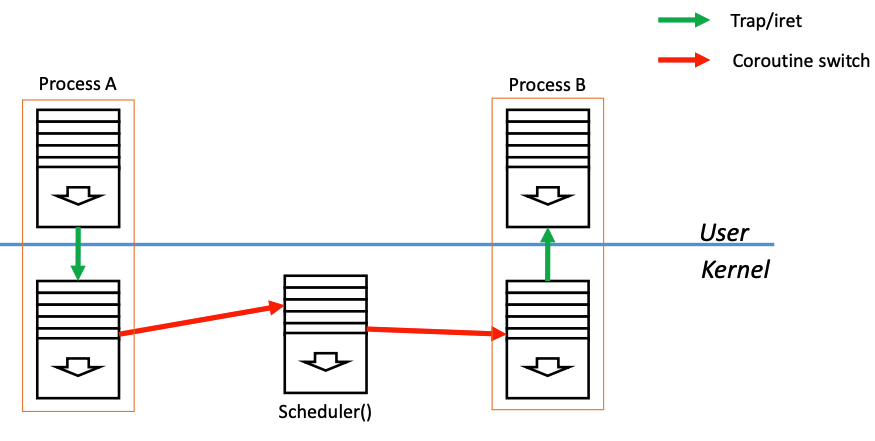
\includegraphics[width=\linewidth]{context-switching.png}
\end{center}


\subsection{Process Hierarchy}

By forking and spawning new processes we create sort of a hierarchy. If a child process dies, but the parent does not call \textit{wait()}, the child process becomes a zombie - it is dead, but still around since nobody asked for the return code. If a parent dies, but the child does not, the child becomes an orphan and gets reparented to the first process (PID \#1, \textit{init}).
\begin{center}
	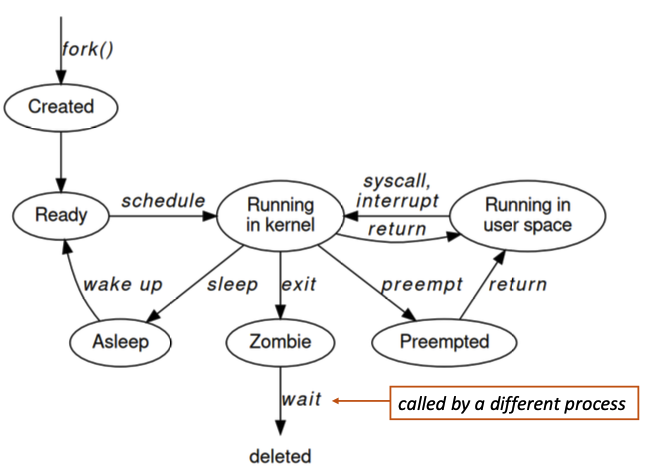
\includegraphics[width=\linewidth]{process-life-cycle.png}
\end{center}

The \textit{init} process is basically an infinite loop calling \textit{wait}(NULL), it gets rid of any zombies.